\subsubsection{Semi-leptonic VV production}
\label{sss-VVprod}

%analysis CMS and ATLAS.
%	[Chatrchyan:2012bd] CMS (7TeV, dijet), Eur. Phys. J. C 73 (2013) 2283, http://arxiv.org/abs/1210.7544 
%	[Chatrchyan:2014aqa] OPTIONAL CMS (8TeV, bjet, (Z(W/Z) -> bb (lv/ll))), Eur. Phys. J. C 74 (2014) 2973, http://arxiv.org/abs/1403.3047 
%	[Aad:2014mda] ATLAS, JHEP01(2015)049, http://arxiv.org/abs/1410.7238


%intro
The cross sections for \WW\; and \WZ\; production have been measured also in the 
semileptonic decay channel in the \WVlvqq\; final state with $\V=\Wpm,\Zzero$.
The semileptonic final state has a relatively large background mainly from \V\; production
with associated jets compared to the fully leptonic decay channels, but offers a 
substantially larger branching fraction. The increased statistics of signal events 
at high partonic centre of mass compared to the fully leptonic 
decay modes enhances specifically the sensitivity to aTGC.
ATLAS and CMS have published measurements of the
inclusive production cross section $\WW+\WZ$ and set limits on charged aTGC 
with the full data set of the $\rts=7\TeV$ run~\cite{Aad:2014mda,Chatrchyan:2012bd}.

%decay channels
Both analysis use the semileptonic decay channel with an electron or muon
and two jets in the final state.
%Selections
The event selection sets requirements 
on the lepton \pT, the \MET, di-jet invariant mass, and the event topology. 
The signal fraction of \WW+\WZ in the event sample after selection is only about 1\%, 
and no further selection criteria are applied to distinguish between 
\WW\; and \WZ\; production.
%Backgrounds
The dominant background from \Z/\W+jets production is constrained with data driven methods,
folowed by the sub-leading background contributions from $\ttbar$ and multi-jet production. 
%systematics
The cross-section is extracted with a simultaneous fit of the di-jet invariant mass 
spectrum comprising the signal and background components. In Figure~\ref{fig:sss-lvjjVVprod-mjj} the di-jet invariant
mass spectrum and the extracted signal after background subtraction from Ref.~\cite{Aad:2014mda} is shown. 
The largest systematic uncertainty is related to the modelling of the \Z/\W+jets background
with about 20\% on the cross section.

\begin{figure}[th!]
  \begin{center}
     \subfigure[]
              {
              %https://atlas.web.cern.ch/Atlas/GROUPS/PHYSICS/PAPERS/STDM-2012-22/fig_03a.pdf
     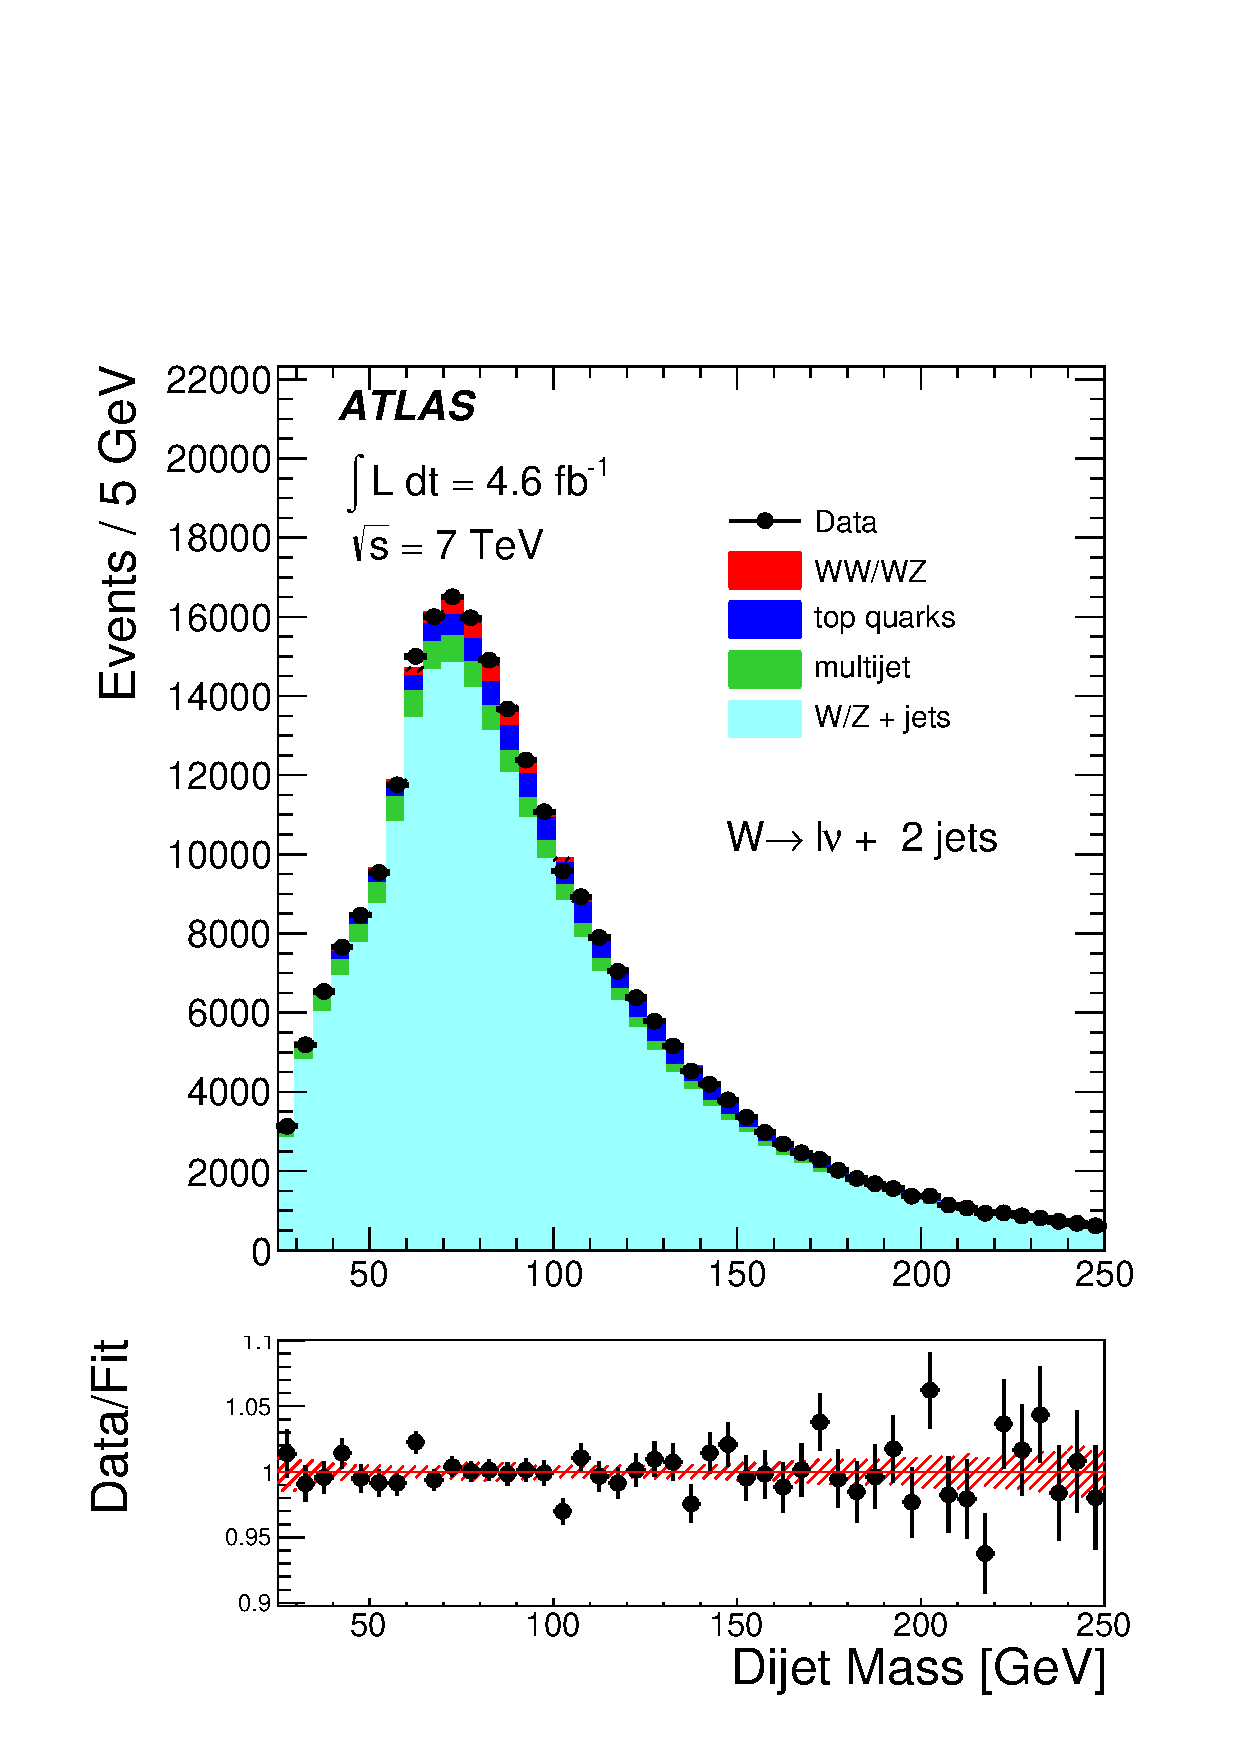
\includegraphics[width=0.485\textwidth]{figures/sss-inclboson-diboson-lvjjVVprod-mjjall.pdf}\label{fig:sss-lvjjVVprod-mjjall}
              }
    \subfigure[]
              {
              %https://atlas.web.cern.ch/Atlas/GROUPS/PHYSICS/PAPERS/STDM-2012-22/fig_03b.pdf
     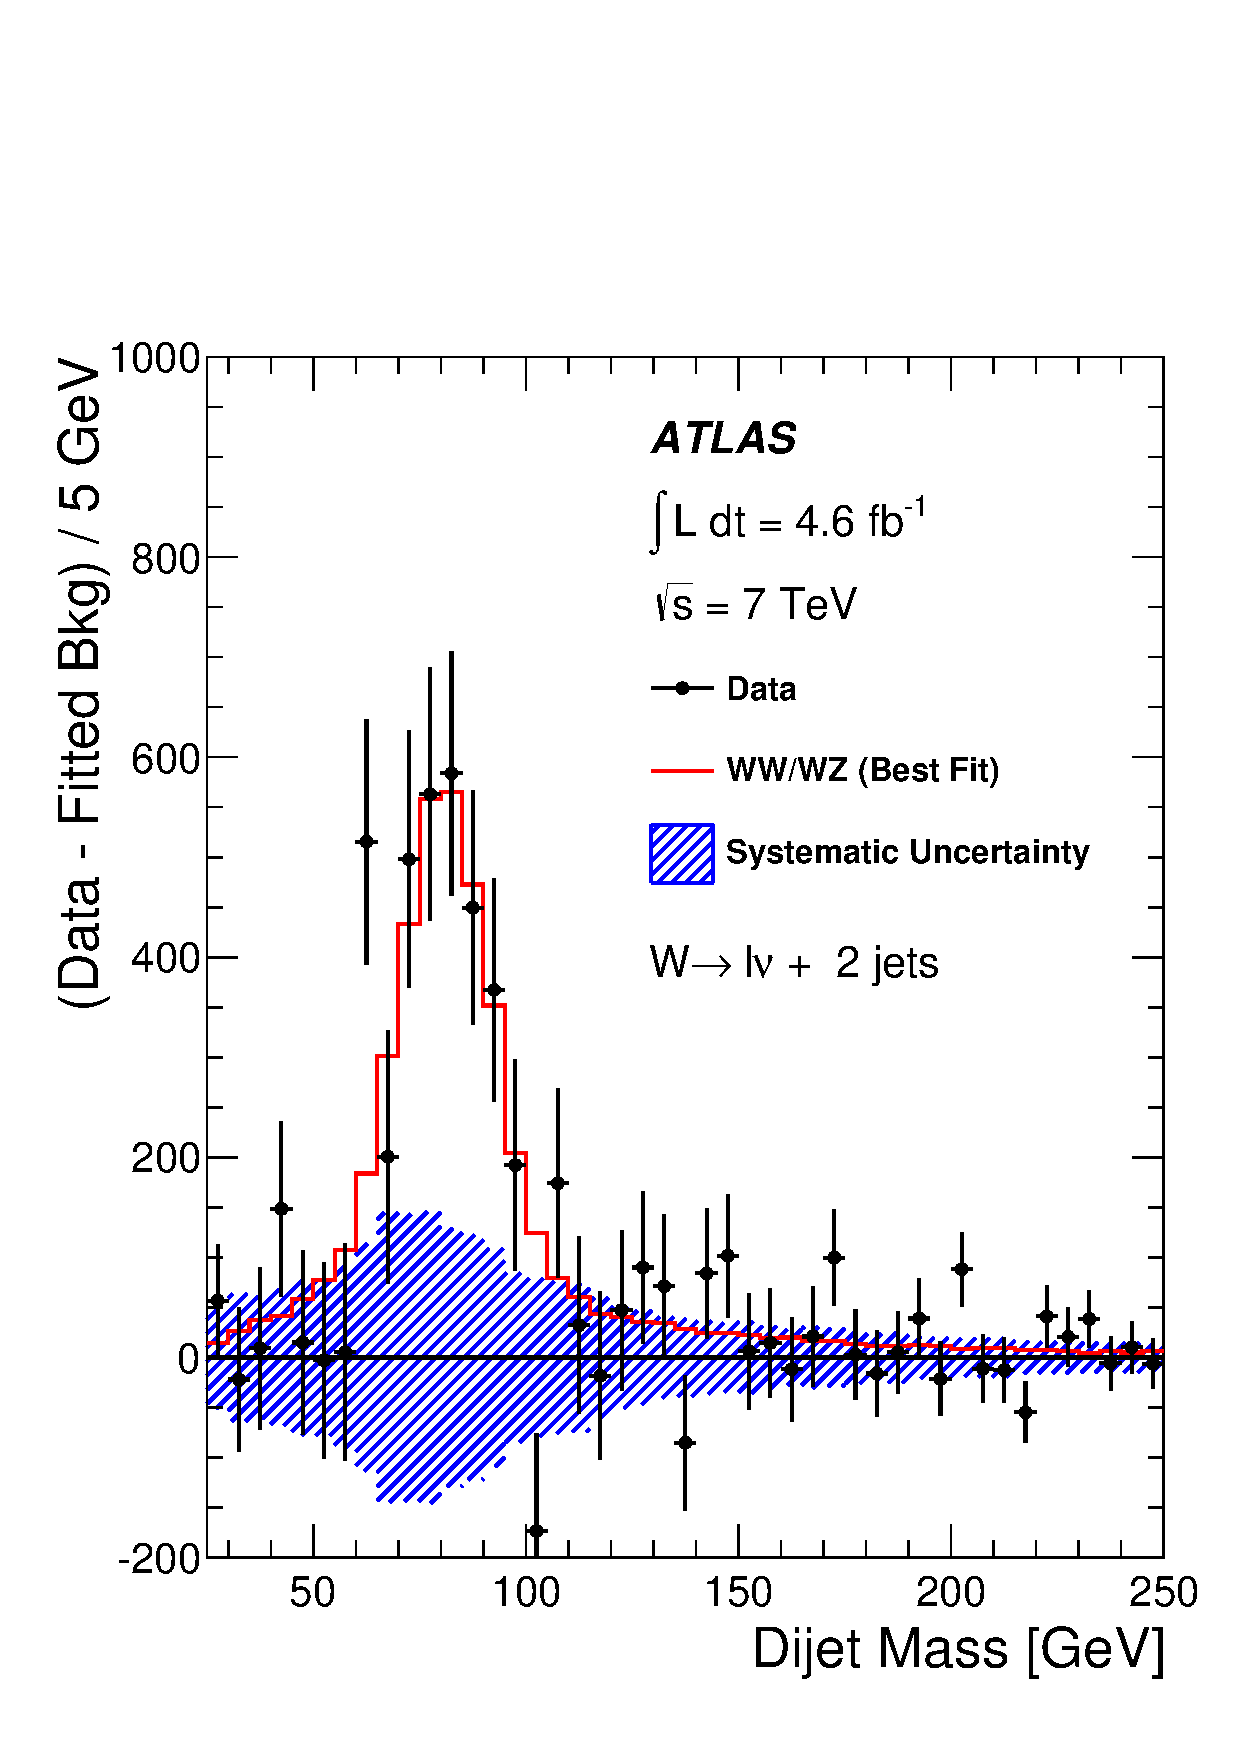
\includegraphics[width=0.485\textwidth]{figures/sss-inclboson-diboson-lvjjVVprod-mjjsig.pdf}\label{fig:sss-lvjjVVprod-mjjsig}
              }
   \end{center}
\vspace{-20 pt}
     \caption{(a) The di-jet invariant mass spectrum for the sum of electron and muon channels, (b) the distribution of the background subtracted data. The lower panel shows that ratio of data and total fit result.}
\label{fig:sss-lvjjVVprod-mjj}
\end{figure}

% Results at the end
The measured and predicted cross sections are compared in Table~\ref{tab:sss-lvjjVVprod-xsec}. 
\begin{table}[htp]
\begin{center}
\resizebox{\textwidth}{!}{
\begin{tabular}{|c|c|c|c|c|c|}
Experiment & cross section & \rts & measured  & predicted  & reference  \\ \hline
ATLAS & total & 7 GeV & {68$\pm{7}$ (stat.) $\pm{19}$ (syst.+lumi.) pb}  & {61.1  $\pm$ ${2.2}$ pb} & \cite{Aad:2014mda} \\
CMS & total & 7 GeV & {68.9 $\pm$ $\pm{8.7}$ (stat.) $\pm{9.7}$ (syst.) $\pm$ 1.5 (lumi.) pb}  & 65.6 $\pm$ 2.2 pb & \cite{Chatrchyan:2012bd} \\
\end{tabular}
}
\caption{Summary of measured total $\WZ+\WW$ production cross sections from ATLAS and CMS
at 7 TeV centre-of-mass energies in the \WVlvqq\; final state.}
\end{center}
\label{tab:sss-lvjjVVprod-xsec}
\end{table}

%TGC
% ATLAS, LEP scenario:
% l_z = l_gamma : obs [-0.039, 0.040], exp [-0.048, 0.047]
% dk_gamma : obs [-0.21,0.22], exp [-0.23,0.25]
% dg1z : obs [-0.055, 0.071], exp [-0.072, 0.085]
%
% CMS: (HISZ, but could be LEP scenario)
% l : obs [-0.038, 0.030]
% dk_gamma : obs [-0.11, 0.14]

To extract limits on aTGC parameters the transverse momentum of the di-jet system $\pt(jj)$ is used 
by ATLAS and CMS. The resulting 95\% CL limits are listed in Table~\ref{tab:sss-lvjjVVprod-ATGC}. The ATLAS
limits use the LEP scenario~\cite{Gounaris:1996rz}, while the CMS limits are derived in the HISZ~\cite{HAGIWARA1992353,PhysRevD.48.2182} scenario. The achieved precision is comparable to the fully leptonic
channel.

\begin{table}\centering
\begin{tabular}{cccc}
\hline
 & CMS & \multicolumn{2}{c}{ATLAS}   \\ 
 & Observed & Observed & Expected \\
\hline
$\lz=\lg$ & $[-0.038, 0.030]$ & $[-0.039, 0.040]$ & $[-0.048, 0.047]$ \\
$\dkg$ 	  & $[-0.11, 0.14]$ & $[-0.21,0.22]$ & $[-0.23,0.25]$ \\
$\dgz$   & \--- & $[-0.055, 0.071]$ & $[-0.072, 0.085]$ \\
\hline
\end{tabular}
\caption{Expected and observed 95\% CL on \dkg, $\lz=\lg$ and \dgz in measured in the 
\WVlvqq\; final state from the ATLAS~\cite{Aad:2014mda} and CMS~\cite{Chatrchyan:2012bd} 
collaborations.}
\label{tab:sss-lvjjVVprod-ATGC}
\end{table}


% mentioning of (Z(W/Z) -> bb (lv/ll))
A  measurement of the \WZ\; and \ZZ\; production cross sections 
at $\rts=8\TeV$ with a data set of $18.9\ifb$ 
in the semileptonic final state with two $b$-quark jets from the \Zzero 
and $\ll$, $\vv$ or $\lnu$ has been published by CMS~\cite{Chatrchyan:2014aqa}, so 
far the only published results at 8 \TeV\; for these channels.
The measured cross sections 
($\sigma(pp\to\WZ)=30.7\pm 9.3$(stat)$\pm 7.1$(syst)$\pm 4.1$(theo)$\pm 1.0$(lumi)$\pb$
and
$\sigma(pp\to\ZZ)=6.5\pm 1.7$(stat)$\pm 1.0$(syst)$\pm 0.9$(theo)$\pm 0.2$(lumi)$\pb$
) 
are consistent with theoretical calculation at
NLO in $\alpha_s$ 
(
$\sigma(pp\to\ZZ) = 22.3\pm 1.1\pb$ and $\sigma(pp\to\ZZ)=7.7\pm 0.4\pb$
), 
with the precision being still statistically limited. 

% unfolded spectra
% https://atlas.web.cern.ch/Atlas/GROUPS/PHYSICS/PAPERS/STDM-2012-01/fig_07.pdf
% 
%\begin{figure}[htbp]
%  \begin{center}
%  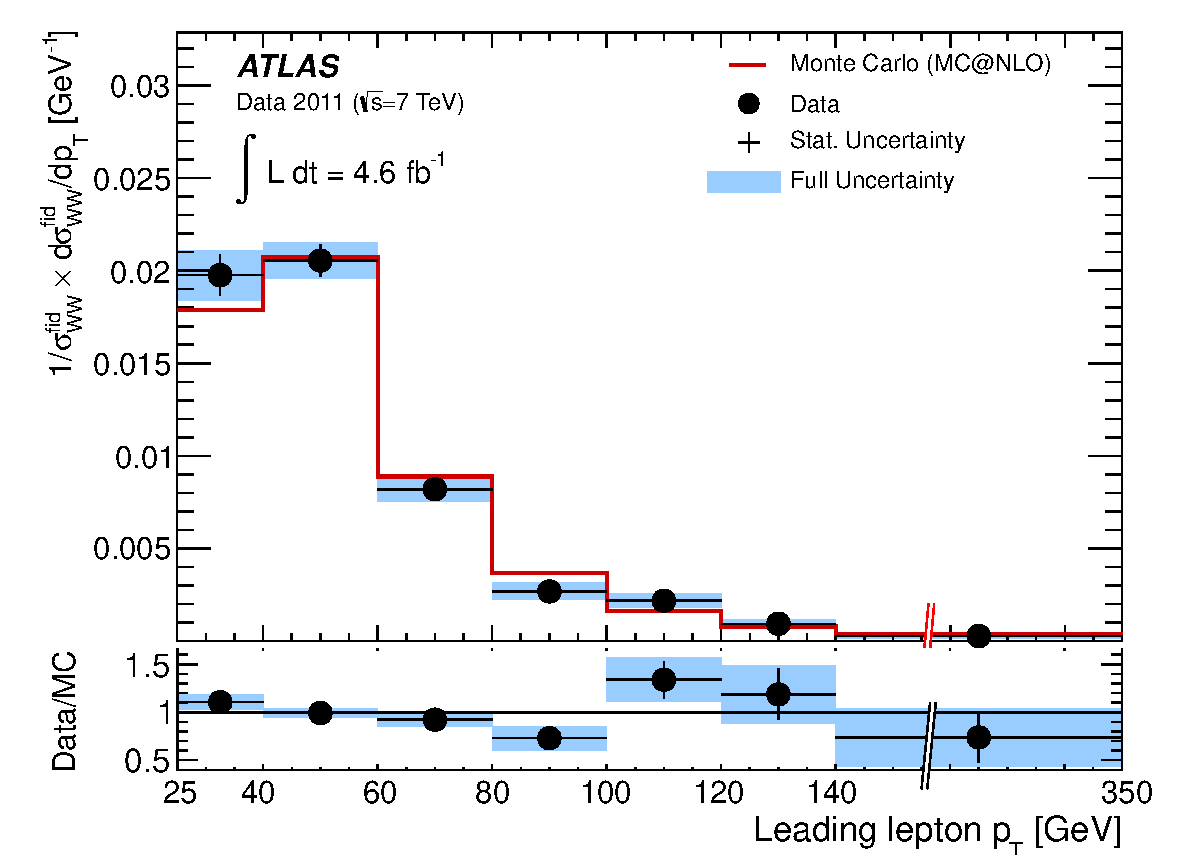
\includegraphics[width=0.45\textwidth]{figures/sss-inclboson-diboson-wwprod-pt-fiducial.pdf}
%  \caption{ATLAS measurement of the transverse momentum of the leading lepton in \WW events compared with the SM prediction at $\rts = 7\TeV$. The full uncertainty contains statistical and systematic uncertainties.}
%\label{fig:sss-WZprod-ptZ}
%\end{center}
%\end{figure}


%%%%
% THIS MIGHT GO INTO THE SECTION ON TGC
% aTGC





